% Workshop paper draft (Springer LNCS format, e.g. ECML-PKDD MLSA).
% Compile on Overleaf (llncs.cls is built in) or locally with: latexmk -pdf main.tex
% Every number in this file comes from docs/results/*.md; figures from paper/make_figures.py.
\documentclass[runningheads]{llncs}

\usepackage[T1]{fontenc}
\usepackage{graphicx}
\usepackage{booktabs}
\usepackage{amsmath}
\usepackage{siunitx}
\usepackage{xcolor}
\usepackage{hyperref}
\newcommand{\todo}[1]{\textcolor{red}{[TODO: #1]}}
\sisetup{group-separator={,}}

\begin{document}

\title{How Much Can You Trust Broadcast Pressing Data?\\
Visibility Bias in Football Tracking Metrics}
\titlerunning{Visibility Bias in Broadcast Pressing Data}

\author{\todo{Author names}}
\authorrunning{\todo{Authors}}
\institute{\todo{Affiliation, email}}

\maketitle

\begin{abstract}
Tracking data derived from broadcast video is cheap and widely available, but the main camera shows only about
14 of the 22 players at a time. We measure how this partial view biases \emph{pressing} metrics. Starting from full
optical tracking of 7 Bundesliga and 2.~Bundesliga matches (and 2 Metrica matches as a replication), we hide every
player a broadcast camera would not show and recompute pressing intensity. The camera is not assumed: we fit a
physical camera model to the on-pitch footprints of 20 real broadcasts (SkillCorner) and validate it on 10 held-out
matches, where it predicts which players are on screen with 87.1\% agreement and reproduces the mean number of
visible players exactly (14.65). Averaged over 20 stadium cameras, broadcast tracking undercounts a team's active
pressers by 22.6\% [95\% CI 19.8, 25.2] (replication: 19.0\% [16.1, 22.0]); for an individual broadcast the
undercount ranges from 10\% to 29\% and is almost perfectly explained by the number of visible players
($r = 0.98$, about 4 percentage points per player). Pressure on the ball carrier is nearly unbiased
($-1.7\%$), but grows with camera lag ($r = -0.98$): even 0.2\,s of lag increases it about fourfold. Both drivers
can be measured on the broadcast itself, which makes the bias correctable. Code and fitted cameras are open source.
\keywords{football \and soccer \and broadcast tracking \and pressing \and measurement bias \and uncertainty}
\end{abstract}

% ---------------------------------------------------------------------------------------------
\section{Introduction}

Pressing, how intensely a team without the ball closes down the opponent, is one of the most discussed tactical
concepts in modern football. Quantifying it requires the positions of all players, which full optical tracking
systems provide but which most clubs, analysts and researchers cannot access. Tracking data extracted from
broadcast video is a much cheaper alternative and is increasingly offered commercially and studied
academically~\cite{somers2024gsr,smf2025broadcast}. Its main limitation is structural: the broadcast camera follows
the action, so players far from the ball are often off screen.

For spatial metrics such as pitch control, this partial view is known to cause large errors in the hidden areas of
the pitch~\cite{offscreen2026}, and several methods impute off-screen players~\cite{omidshafiei2022graphimputer,%
rsos2025continuous,offscreen2026}. For pressing metrics the size of the bias, what drives it, and how certain we can
be about it have not been measured. Because pressing is defined by defenders \emph{near} the ball and also by those
covering passing lanes further away, it is not obvious whether a ball-following camera biases it at all.

We answer three questions:
\begin{enumerate}
\item \textbf{How large is the visibility bias in pressing metrics?} We compare pressing intensity~\cite{bekkers2025pressing}
on full tracking with the same metric after hiding off-screen players.
\item \textbf{How certain is it?} We propagate three sources of uncertainty: the matches in the sample, variation within
a match, and differences between stadium cameras.
\item \textbf{What drives it?} We relate the bias to measurable properties of the broadcast.
\end{enumerate}

\noindent Our contributions are:
(i) a physical broadcast-camera model fitted to and validated on the footprints of 20 real broadcasts, which
outperforms the common rectangular approximation and shows that camera operators frame the players, not only the ball;
(ii) the first measurement, to our knowledge, of visibility bias in pressing metrics, with confidence intervals that include
stadium-to-stadium camera variation and a replication on a second data provider;
(iii) the finding that the bias is almost fully explained by two quantities measurable on the broadcast, the number of
visible players and camera lag; and
(iv) an open-source implementation of the full pipeline. \todo{Novelty claim to be re-checked against recent literature
before submission.}

% ---------------------------------------------------------------------------------------------
\section{Related Work}

\textbf{Broadcast tracking.} SoccerNet Game State Reconstruction~\cite{somers2024gsr} benchmarks the extraction of
player positions on a minimap from broadcast video; commercial providers deliver broadcast tracking at scale
(e.g.\ SkillCorner~\cite{skillcorner_opendata}). The reliability of broadcast-derived data for analytics was studied
in~\cite{smf2025broadcast}. \todo{Summarise its findings after reading it in full.}

\textbf{Off-screen players.} Graph Imputer~\cite{omidshafiei2022graphimputer} predicts the trajectories of off-screen
players; \cite{rsos2025continuous} builds continuous tracks from discrete broadcast data. Closest to our work,
\cite{offscreen2026} simulates a broadcast camera on Metrica data and reports large pitch-control errors in hidden
zones, together with a training-free imputation method. \todo{Verify this description against the full paper; contrast
their camera simulation with our fitted camera.} We study pressing rather than pitch control, fit the camera to real
footprints instead of assuming it, and quantify uncertainty including camera variation.

\textbf{Pressing.} We use the pressing intensity of Bekkers~\cite{bekkers2025pressing}, which gives, for every
defender--attacker pair, the probability that the defender can intercept the attacker within a time threshold, based
on positions and velocities. Related spatial models include pitch control~\cite{spearman2018beyond}.

% ---------------------------------------------------------------------------------------------
\section{Data}

\textbf{Ground truth.} The IDSSE open dataset~\cite{bassek2025idsse} (CC-BY 4.0) contains optical tracking of all
22 players and the ball at 25\,Hz for 7 matches of the 2022/23 Bundesliga and 2.~Bundesliga, with possession
information. After keeping ball-in-play frames, 552{,}294 frames remain. As a replication we use the 2 Metrica Sports
sample games~\cite{metrica_sample} (25\,Hz, all players), for which we reconstruct possession and ball-in-play status
from the accompanying event file (166{,}913 frames). \todo{Note: one team appears in 5 of the 7 IDSSE matches.}

\textbf{Real broadcasts.} The SkillCorner open data~\cite{skillcorner_opendata} (MIT licence) contains broadcast
tracking of 20 A-League 2024/25 matches at 10\,Hz. For every frame it gives the four corners of the camera image
projected onto the pitch, and for every player whether they were detected on screen or extrapolated. We use it only to
fit and validate the camera model (375{,}357 frames for fitting).

% ---------------------------------------------------------------------------------------------
\section{Method}

\subsection{Pressing metrics}
For each frame with a ball carrier we compute the matrix $P$ of interception probabilities between defenders
(rows) and attackers (columns) with \texttt{unravelsports}~\cite{unravelsports} (speed threshold 2\,m/s). We report
two summaries per frame:
\emph{pressure on the ball carrier}, $1 - \prod_i (1 - P_{i,c})$ over defenders $i$ for carrier $c$, a local metric; and
the number of \emph{active pressers}, defenders whose largest probability exceeds 0.5, a team-wide metric.
Frames without a ball carrier in the possessing team (0.06--0.2\% per match) are dropped.

\subsection{Simulating the broadcast view}
Given full tracking and a camera model, we remove every player outside the camera's view and recompute the metrics
on the remaining players; the ball and the ball carrier are always kept. A frame in which no defender is visible
counts as zero pressure. The bias of a metric is the relative difference between the mean over a team's
out-of-possession frames with and without hiding.

\textbf{Rectangle camera (baseline).} A window of fixed length along the pitch (full width), centred on the ball and
clipped to the pitch, as commonly assumed. A 40\,m window shows 14.5 players on average.

\textbf{Wedge camera (fitted).} The main camera is a fixed point $(c_x, c_y)$ behind the near touchline. A player at
bearing $\theta$ from the camera is visible if $|\theta - \phi_t| \le \alpha_t/2$ and their depth along the viewing
direction exceeds the bottom image edge $\nu_t$:
\begin{align}
\phi_t &= \mathrm{EMA}_{\lambda}\!\left(g_b\,\theta^{\text{ball}}_t + g_p\,\bar\theta^{\text{players}}_t + o\right),\\
\alpha_t &= \mathrm{clip}\!\left(a_0 + a_1 d^{\text{ball}}_t + a_2\, s^{\text{players}}_t\right),\qquad
\nu_t = n_0 + n_1 d^{\text{ball}}_t,
\end{align}
where $\phi$ is the pan, $\alpha$ the horizontal field of view, $d^{\text{ball}}$ the ball's distance from the camera,
$\bar\theta^{\text{players}}$ and $s^{\text{players}}$ the mean and standard deviation of the players' bearings, and
$\lambda$ an exponential lag (time constant).

\subsection{Fitting and validating the camera}
In every SkillCorner frame, the left and right image edges are rays from the camera's ground position; their
intersection locates the camera (median per match). Pan and field of view follow from the bearings of the far image
corners, the bottom edge from the near corners. We fit $(g_b, g_p, o)$, $(a_0,a_1,a_2)$ and $(n_0,n_1)$ by least
squares and $\lambda$ by grid search (0--1\,s). We fit one shared camera on 10 matches and test it on the other 10,
comparing predicted visibility with the per-player \texttt{is\_detected} flags; the real footprint itself gives an
upper bound. To capture stadium differences we also fit one camera per match (20 cameras).

\subsection{Uncertainty}
Frames 40\,ms apart are strongly dependent, so we use a block bootstrap with 60\,s blocks within each team-match. For a
single camera, a two-level bootstrap resamples matches (both teams together) and blocks. Across stadium cameras, a
three-level bootstrap additionally resamples the 20 cameras; we report intervals for each source alone and combined
(2{,}000 replicates, 95\% percentile intervals). For the 20-camera runs, metrics are evaluated every 0.2\,s while the
camera follows every frame; this changes the bias by less than 0.1 percentage points (checked on one full match).

% ---------------------------------------------------------------------------------------------
\section{Results}

\subsection{A camera fitted to real broadcasts}

\begin{figure}[t]
\centering
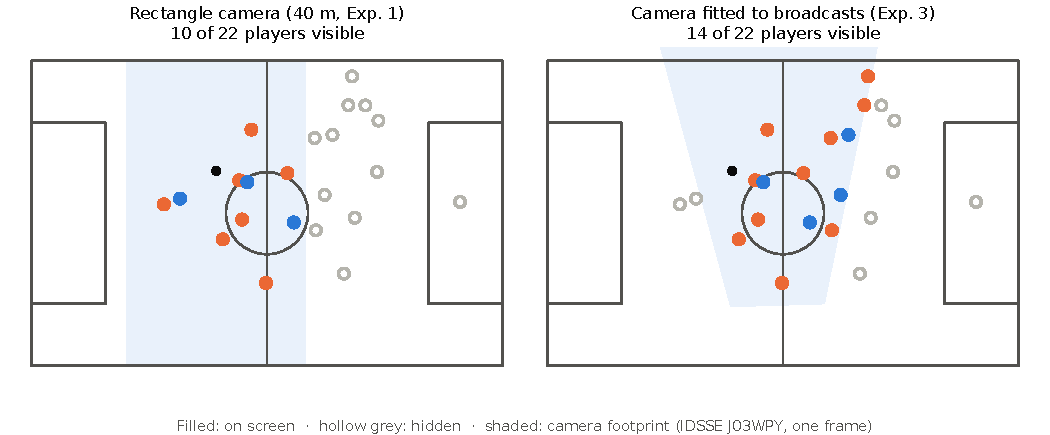
\includegraphics[width=\textwidth]{figures/fig1_cameras.pdf}
\caption{The same IDSSE frame seen by the rectangle camera (left) and the camera fitted to real broadcasts (right).
The fitted camera stands behind the near touchline: its footprint widens towards the far side and cuts off players
close to the camera.}
\label{fig:cameras}
\end{figure}

The fitted camera stands on the halfway line, 57--97\,m from the pitch centre depending on the stadium. Its pan
follows the ball and the players' centre with similar weights ($g_b = 0.57$, $g_p = 0.56$; $R^2 = 0.97$) and
\textbf{without measurable lag} (best $\lambda = 0$\,s for the shared camera). The median field of view is 27°
(19--40°): it narrows when play is far away and widens when players are spread ($R^2 = 0.48$); the bottom edge moves
away with the ball ($R^2 = 0.60$). Figure~\ref{fig:cameras} shows the resulting footprint.

\begin{table}[t]
\centering
\caption{Which players are on screen? Agreement of each camera model with SkillCorner's per-player detection flags on
10 held-out matches.}
\label{tab:validation}
\begin{tabular}{lcc}
\toprule
Camera model & Agreement & Visible players / frame \\
\midrule
Real footprint (upper bound) & 96.8\% & -- \\
\textbf{Fitted wedge camera} & \textbf{87.1\%} & \textbf{14.65} \\
Rectangle, 40\,m & 82.9\% & 15.76 \\
Rectangle, 32\,m with assumed lag, perspective, zoom & 82.2\% & 15.29 \\
Wedge camera following the ball only & 82.0\% & 13.30 \\
\midrule
Real broadcast & -- & 14.65 \\
\bottomrule
\end{tabular}
\end{table}

Table~\ref{tab:validation} shows that the fitted camera beats the rectangle on all 10 held-out matches (84.0--88.9\%
per match vs.\ 79.5--86.1\%) and reproduces the mean number of visible players exactly. Following only the ball
underestimates visibility; adding random framing noise also made predictions worse (80.7\%), so it is not used.

\subsection{Visibility bias in pressing metrics}

\begin{table}[t]
\centering
\caption{Relative bias of pressing metrics under different cameras (negative = undercount). 95\% block-bootstrap
intervals; the stadium ensemble interval includes camera, match and within-match variation.}
\label{tab:bias}
\setlength{\tabcolsep}{4pt}
\begin{tabular}{llccc}
\toprule
Data & Camera & Visible & Pressure on carrier & Active pressers \\
\midrule
IDSSE & Rectangle 40\,m & 14.5 & $-0.1\%$ [$-0.2$, $-0.1$] & $-20.3\%$ [$-22.7$, $-17.9$] \\
IDSSE & Rectangle 40\,m, assumed 0.5\,s lag & 14.3 & $-4.1\%$ [$-4.6$, $-3.7$] & $-24.1\%$ [$-26.5$, $-21.9$] \\
IDSSE & Fitted shared camera & 13.8 & $-0.5\%$ [$-0.7$, $-0.4$] & $-21.4\%$ [$-23.8$, $-19.1$] \\
IDSSE & \textbf{20 stadium cameras} & 12.1--16.0 & $\mathbf{-1.7\%}$ [$-2.2$, $-1.2$] & $\mathbf{-22.6\%}$ [$-25.2$, $-19.8$] \\
\midrule
Metrica & Fitted shared camera & 14.5 & $-0.7\%$ [$-1.0$, $-0.5$] & $-17.7\%$ [$-20.8$, $-15.1$] \\
Metrica & \textbf{20 stadium cameras} & 12.8--16.6 & $\mathbf{-1.8\%}$ [$-2.3$, $-1.3$] & $\mathbf{-19.0\%}$ [$-22.0$, $-16.1$] \\
\bottomrule
\end{tabular}
\end{table}

Table~\ref{tab:bias} summarises the main result. With every camera model, broadcast tracking undercounts a team's
active pressers by about one fifth: 22.6\% on IDSSE and 19.0\% on Metrica when averaged over the 20 stadium cameras.
No per-team interval contains zero (fitted shared camera, IDSSE: $-16\%$ to $-27\%$ per team), and the ranking of
teams by active pressers is largely but not fully preserved (Spearman $\rho = 0.90$). Pressure on the ball carrier is much
less affected ($-0.5\%$ to $-1.8\%$). The stadium camera alone contributes as much uncertainty as the sample of matches
(IDSSE, active pressers: camera only [$-24.3$, $-20.6$], matches and blocks only [$-24.4$, $-20.6$]).

\textbf{Replication.} The same camera shows about one more player on Metrica than on IDSSE (more compact teams).
At equal visibility the two data sources agree closely: with the assumed-lag rectangle camera tuned to 14.5 visible
players,
active pressers are undercounted by 22.3\% [19.6, 25.3] on Metrica and 22.8\% [20.5, 25.1] on IDSSE.
\todo{This comparison uses the assumed-lag rectangle of Exp.~1b; repeat with the fitted camera.}

\subsection{What drives the bias}

\begin{figure}[t]
\centering
\begin{minipage}{0.49\textwidth}\centering
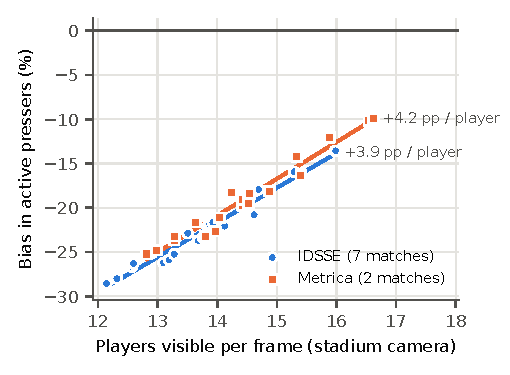
\includegraphics[width=\linewidth]{figures/fig2_visibility.pdf}
\end{minipage}\hfill
\begin{minipage}{0.49\textwidth}\centering
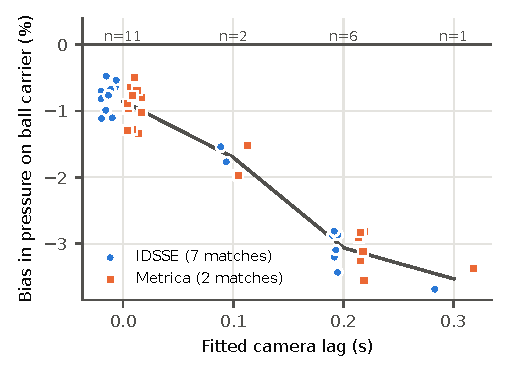
\includegraphics[width=\linewidth]{figures/fig3_lag.pdf}
\end{minipage}
\caption{One point per stadium camera and dataset. Left: the undercount of active pressers shrinks by about
4 percentage points per additional visible player ($r = 0.98$). Right: the bias in pressure on the ball carrier grows
with the camera's fitted lag ($r = -0.98$); $n$ = number of stadium cameras per lag value.}
\label{fig:drivers}
\end{figure}

Across stadium cameras, the bias is almost fully explained by two properties of the broadcast
(Fig.~\ref{fig:drivers}). For active pressers it is the \textbf{number of visible players}: broadcasters that frame the
whole group (15--16 players visible) miss about 13\%, tight framing (about 12 visible) up to 29\% ($r = 0.98$; slope
3.9 and 4.2 percentage points per player on IDSSE and Metrica). For pressure on the ball carrier it is \textbf{camera
lag}: 11 of 20 stadium cameras show no measurable lag ($-0.8\%$), 0.1\,s gives $-1.7\%$, 0.2\,s $-3.1\%$ and
0.3\,s $-3.7\%$ ($r = -0.98$). Defenders closing down the carrier enter the picture late when the camera trails the ball.
The shared camera averages these lags away, which is why it shows a smaller carrier bias. An assumed lag of 0.5\,s, as
in our initial rectangle experiments, overstates the carrier bias (Table~\ref{tab:bias}).

% ---------------------------------------------------------------------------------------------
\section{Discussion}

\textbf{Implications.} Carrier-centred pressing metrics can be used on broadcast data with small error, provided the
camera does not lag. Team-wide pressing metrics, such as the number of players involved in a press, are undercounted by
about one fifth on average and by up to 29\% for tightly framed broadcasts. Comparing teams or matches filmed with
different camera styles can therefore be misleading.

\textbf{Correction.} Because both drivers, visible players and camera lag, can be measured on the broadcast itself,
a simple correction is possible: estimate the expected undercount from the per-frame number of visible players and
rescale. \todo{Fit and validate the correction with leave-one-stadium-out evaluation (next step).}

\textbf{Limitations.} The ground truth covers 9 matches from two sources, with one team in 5 of the 7 IDSSE matches.
The camera is fitted on A-League broadcasts; other leagues may be filmed differently. SkillCorner's detection flags
also reflect detector errors, which caps agreement at about 97\%. Per-stadium cameras are fitted and evaluated on the
same match (the held-out test uses the shared camera). We simulate only the main camera; replays, close-ups and
camera cuts are not modelled. Metrica possession is reconstructed from hand-annotated events.

% ---------------------------------------------------------------------------------------------
\section{Conclusion}

Using a broadcast camera fitted to and validated on real footage, we showed that broadcast tracking undercounts a
team's active pressers by about one fifth (22.6\% [19.8, 25.2]), robustly across matches, stadium cameras and a second
data provider, while pressure on the ball carrier is nearly unbiased unless the camera lags. Both effects are almost
fully explained by quantities measurable on the broadcast, which opens the way to correcting broadcast pressing metrics.

\subsubsection*{Data and code availability.}
Code, fitted camera parameters and scripts to rebuild every table and figure: \cite{pitchlens}. Data are downloaded
from their original sources and not redistributed. We thank IDSSE (Bassek et al.), Metrica Sports and SkillCorner for
making their data openly available.

\bibliographystyle{splncs04}
\bibliography{refs}

\end{document}
